\documentclass[a4paper, 11pt]{article}
\usepackage[UTF8, scheme = plain]{ctex}
\usepackage{amsmath}
\usepackage{graphicx}
\usepackage{geometry}
\usepackage{listings}
\geometry{scale=0.8}
\linespread{1.5}
\usepackage{hyperref}
\usepackage{listings}
\usepackage{enumitem}
\setenumerate[1]{itemsep=0pt,partopsep=0pt,parsep=\parskip,topsep=0pt}
\setitemize[1]{itemsep=0pt,partopsep=0pt,parsep=\parskip,topsep=0pt}
\setdescription{itemsep=0pt,partopsep=0pt,parsep=\parskip,topsep=0pt}


\title{	
\normalfont \normalsize
\textsc{School of Data and Computer Science, Sun Yat-sen University} \\ [25pt] %textsc small capital letters
\rule{\textwidth}{-1.5pt} \\[0.4cm] % Thin top horizontal rule
\huge  E10 Decision Tree\\ % The assignment title
\rule{\textwidth}{2pt} \\[0.5cm] % Thick bottom horizontal rule
\author{20214810 Suixin Ou\and20214966 Yangkai Lin}
\date{\normalsize November 16, 2020} 
}

\begin{document}
\maketitle
\tableofcontents
\newpage

\section{Datasets}
\label{sec:datasets}

The UCI dataset (\url{http://archive.ics.uci.edu/ml/index.php}) is the most widely used dataset for machine learning. If you are interested in other datasets in other areas, you can refer to \url{https://www.zhihu.com/question/63383992/answer/222718972}.

Today's experiment is conducted with the \textbf{Adult Data Set} which can be found in \url{http://archive.ics.uci.edu/ml/datasets/Adult}. 
\begin{figure}[ht]
\centering
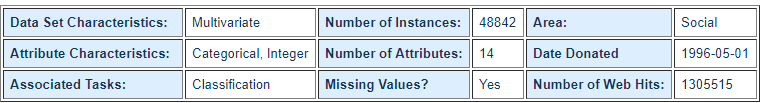
\includegraphics[width=17cm]{dataset.png}
\end{figure}

You can also find 3 related files in the current folder, \texttt{adult.name} is the description of \textbf{Adult Data Set}, \texttt{adult.data} is the training set, and \texttt{adult.test} is the testing set. There are 14 attributes in this dataset:
\begin{lstlisting}{language=Python}
>50K, <=50K.

1. age: continuous.
2. workclass: Private, Self-emp-not-inc, Self-emp-inc, Federal-gov, Local-gov, 
State-gov, Without-pay, Never-worked.
3. fnlwgt: continuous.
4. education: Bachelors, Some-college, 11th, HS-grad, Prof-school, Assoc-acdm, 
Assoc-voc, 9th, 7th-8th, 12th, Masters, 5. 1st-4th, 10th, Doctorate, 5th-6th, 
Preschool.
5. education-num: continuous.
6. marital-status: Married-civ-spouse, Divorced, Never-married, Separated, 
Widowed, Married-spouse-absent, Married-AF-spouse.
7. occupation: Tech-support, Craft-repair, Other-service, Sales, 
Exec-managerial, Prof-specialty, Handlers-cleaners, Machine-op-inspct, 
Adm-clerical,Farming-fishing,Transport-moving,Priv-house-serv,Protective-serv, 
Armed-Forces.
8. relationship: Wife,Own-child,Husband,Not-in-family,Other-relative,Unmarried.
9. race: White, Asian-Pac-Islander, Amer-Indian-Eskimo, Other, Black.
10. sex: Female, Male.
11. capital-gain: continuous.
12. capital-loss: continuous.
13. hours-per-week: continuous.
14. native-country: United-States, Cambodia,England,Puerto-Rico,Canada,Germany, 
Outlying-US(Guam-USVI-etc),India,Japan,Greece, South,China,Cuba,Iran,Honduras, 
Philippines, Italy, Poland, Jamaica, Vietnam, Mexico, Portugal, Ireland, France, 
Dominican-Republic,Laos,Ecuador,Taiwan, Haiti, Columbia,Hungary,Guatemala, 
Nicaragua,Scotland,Thailand,Yugoslavia,El-Salvador, Trinadad&Tobago,Peru,Hong, 
Holand-Netherlands.

\end{lstlisting}
\textbf{Prediction task is to determine whether a person makes over 50K a year.}

\section{Decision Tree}

\subsection{ID3}
ID3 (Iterative Dichotomiser 3) was developed in 1986 by Ross Quinlan. The algorithm creates a multiway tree, finding for each node (i.e. in a greedy manner) the categorical feature that will yield the largest information gain for categorical targets. Trees are grown to their maximum size and then a pruning step is usually applied to improve the ability of the tree to generalise to unseen data.

\textbf{ID3 Algorithm:}
\begin{enumerate}
	\item Begins with the original set $S$ as the root node.
	\item Calculate the entropy of every attribute $a$ of the data set $S$.
	\item Partition the set $S$ into subsets using the attribute for which the resulting entropy after splitting is minimized; or, equivalently, information gain is maximum.
	\item Make a decision tree node containing that attribute.
	\item Recur on subsets using remaining attributes.
\end{enumerate}

\textbf{Recursion on a subset may stop in one of these cases:}
\begin{itemize}
	\item every element in the subset belongs to the same class; in which case the node is turned into a leaf node and labelled with the class of the examples.
	\item there are no more attributes to be selected, but the examples still do not belong to the same class. In this case, the node is made a leaf node and labelled with the most common class of the examples in the subset.
	\item there are no examples in the subset, which happens when no example in the parent set was found to match a specific value of the selected attribute. 
\end{itemize}

\textbf{ID3 shortcomings:}
\begin{itemize}
	\item ID3 does not guarantee an optimal solution. 
	\item ID3 can overfit the training data. 
	\item ID3 is harder to use on continuous data.
\end{itemize}

\textbf{Entropy:}

Entropy $H(S)$ is a measure of the amount of uncertainty in the set $S$.
$$H(S)=\sum_{x\in X}-p(x)\log_2p(x)$$
where
\begin{itemize}
	\item $S$ is the current dataset for which entropy is being calculated
	\item $X$ is the set of classes in $S$
	\item $p(x)$ is the proportion of the number of elements in class $x$ to the number of elements in set $S$.
\end{itemize}

\textbf{Information gain:}

Information gain $IG(A)$ is the measure of the difference in entropy from before to after the set $S$ is split on an attribute $A$. In other words, how much uncertainty in $S$ was reduced after splitting set $S$ on attribute $A$.
$$IG(S,A)=H(S)-\sum_{t\in T}p(t)H(t)=H(S)-H(S\ |\ A)$$
where
\begin{itemize}
	\item $H(S)$ is the entropy of set $S$
	\item T is the subsets created from splitting set $S$ by attribute $A$ such that $S=\cup_{t\in T}t$
	\item $p(t)$ is the proportion of the number of elements in $t$ to the number of elements in set $S$
	\item $H(t)$ is the entropy of subset $t$.
\end{itemize}
\subsection{C4.5 and CART}
C4.5 is the successor to ID3 and removed the restriction that features must be categorical by dynamically defining a discrete attribute (based on numerical variables) that partitions the continuous attribute value into a discrete set of intervals. C4.5 converts the trained trees (i.e. the output of the ID3 algorithm) into sets of if-then rules. These accuracy of each rule is then evaluated to determine the order in which they should be applied. Pruning is done by removing a rule’s precondition if the accuracy of the rule improves without it.

C5.0 is Quinlan’s latest version release under a proprietary license. It uses less memory and builds smaller rulesets than C4.5 while being more accurate.

CART (Classification and Regression Trees) is very similar to C4.5, but it differs in that it supports numerical target variables (regression) and does not compute rule sets. CART constructs binary trees using the feature and threshold that yield the largest information gain at each node.


\section{Tasks}
\begin{itemize}
\item Given the training dataset \texttt{adult.data} and the testing dataset \texttt{adult.test}, please accomplish the prediction task to determine whether a person makes over 50K a year in \texttt{adult.test} by using ID3 (or C4.5, CART) algorithm (C++ or Python), and compute the accuracy. 
\begin{enumerate}
\item You can process the continuous data with \textbf{bi-partition} method.
\item You can use prepruning or postpruning to avoid the overfitting problem.
\item You can assign probability weights to solve the missing attributes (data) problem.
\end{enumerate}

\item Please finish the experimental report named \texttt{E10\_YourNumber.pdf}, and send it to \texttt{ai\_2020@foxmail.com}
\end{itemize}

\section{Codes and Results}
\subsection{Codes}
我实现了运用信息增益作为\textbf{IMPORTANCE}的ID3
和运用信息增益比作为\textbf{IMPORTANCE}的C4.5
(不过是贪婪的选信息增益比最大的)。
连续数据方面我采用一个半成的\textbf{bi-partition}方法,
和\textbf{bi-partitioin}方法。
剪枝方面我实现了预剪枝。
缺失值处理缺省是直接忽略,
也实现了赋予权重。
\textbf{DECISION\_TREE\_LEARNING}的实现,
参考了理论课课件的伪代码,并做了一些优化。
其他实现均参考
\url{https://blog.csdn.net/u012328159/article/details/70184415}
系列博客。

\subsubsection{PLURALITY\_VALUE}
函数作用是返回\textbf{examples}中最大的\textbf{classification},
作为\textbf{DECISION\_TREE\_LEARNING}几种递归终止的返回值。
同时判断是否只有一种\textbf{classification},
对应\textbf{DECISION\_TREE\_LEARNING}的一种递归终止条件的判断。

\subsubsection{IMPORTANCE}
信息熵用\textbf{B}计算,
里面使用了判断用于计算参数$q=0$或$q=1$的情况,
由于后面引入权重,用浮点数计算精度受限可能会出现$q>1$的情况,
所以用不等式判断。
\begin{lstlisting}[language=python]
if q <= 0 or q >= 1:
	return 0.0
\end{lstlisting}

信息增益用\textbf{INFORMATION\_COUNT}配合\textbf{GAIN}计算,
信息增益比用\textbf{INFORMATION\_COUNT}配合\textbf{GAIN\_RATIO}计算。
信息增益比类似于对信息增益的归一化处理,不会偏好可取值多的属性,但
会偏好可取值少的属性。

\subsubsection{Missing Data}
\textbf{WEIGHTING}根据属性\textbf{A}的不同取值将\textbf{examples}
分成\textbf{exs\_dict}。先分非缺失值,对于缺失值,
以不同集合的大小为权重,
\begin{lstlisting}[language=python]
if total_weight != 0:
	weight = example.weight * weights[vk] / total_weight
else:
	weight = example.weight / len(examples)
\end{lstlisting}
将一个含缺失值的\textbf{example}分给每一个集合。
\begin{lstlisting}[language=python]
exs_dict[vk].append(Example(example.attributes, example.classification, weight))
\end{lstlisting}
对于训练集缺失值处理在\textbf{INFORMATION\_COUNT}也有,
因为是用于计算分前后信息熵变化,所以处理类似。

以上都是对训练集的缺失值的处理,下面是对测试集的缺失值的处理。

\textbf{DECISION\_TREE\_PREDICTING}函数用于对于\textbf{attributes}
给出\textbf{predict}。这里定义\textbf{predict}是
\textbf{[(classification, weight)]}格式的,
\textbf{weight}可以理解成预测该分类的概率。
在树上寻路过程中,遇到缺失值,按照每条分支的权重(训练时由每条分支的
对应集合的权重和除以所有分支的集合权重和)产生分叉,
\begin{lstlisting}[language=python]
if value == '?':
	for new_classification, new_weight in classification.branches.values():
		stack.append((new_classification, weight * new_weight))
\end{lstlisting}
就从遍历一条路径问题变成了遍历一个树,因而通过维护一个\textbf{Frontier}如\textbf{stack}即可。
\begin{lstlisting}[language=python]
predict = list()
stack = [(tree, 1)]
while len(stack) > 0:
	classification, weight = stack.pop()
	if type(classification) == DecisionTree:
		pass
	else:
		predict.append((classification, weight))
\end{lstlisting}

\subsubsection{Pruning}
\textbf{CLASSIFICATION\_COUNT}用于计数一个\textbf{examples}中
\textbf{classification}出现次数。
剪枝需要先将训练集分为训练集和验证集(默认7:3分),
\begin{lstlisting}[language=python]
if preprune is True and validating_examples is None:
	random.shuffle(training_examples)
	split_point = int(len(training_examples) * split_point)
	validating_examples = training_examples[split_point:]
	training_examples = training_examples[:split_point]
\end{lstlisting}
然后用训练集选属性\textbf{A},并用\textbf{A}分训练集,
再用验证集验证这样分是熵减的。
\begin{lstlisting}[language=python]
if preprune is True:
	last_right = CLASSIFICATION_COUNT(plurality_value, validating_examples)
	WEIGHTING(exs_vali_dict, A, validating_examples)
	right = 0
	for exs in exs_vali_dict.values():
		if len(exs) != 0:
			right += CLASSIFICATION_COUNT(PLURALITY_VALUE(exs)[0], exs)
	if last_right >= right:
		return plurality_value
\end{lstlisting}
这样不仅可以增强模型泛用性(模型过于复杂容易出现过拟合的问题),
而且可以减少训练时间(提前剪枝,不用考虑后面的)。

另外后剪枝和其类似,实际上是把这步判断在最后返回树前进行,与预剪枝
相比,好处是建完整棵树后再递归地剪枝,不会像预剪枝一样不继续分支而
导致丢失一些信息,坏处是比预剪枝慢。

\subsubsection{Continuous Data}
该部分涉及以下四个函数
\begin{enumerate}
	\item \textbf{GAIN\_FOR\_BI\_PARTITION},
	一个方便使用的信息增益变体。
	\item \textbf{CONTINUOUS\_VALUE\_PROCESSING},
	连续值处理的主体。
	\item \textbf{TRAINING\_EXAMPLES\_UPDATE},
	对训练集应用连续值处理。
	\item \textbf{DECISION\_TREE\_TESTING},
	包含对测试集应用连续值处理。
\end{enumerate}

首先是二分法的半成品,思路其实就是用训练集中连续属性相邻连续值的中点
构成区间转换成离散属性。优点是处理快且实现简单,缺点是训练慢且
树过于复杂容易过拟合且取值过多,容易导致偏好取值多的信息增益和偏好
取值少的信息增益比的一方出现严重问题。

然后是二分法,是在二分法半成品的基础上,选一个分后熵减最大的点,
将连续属性转化成只有两种取值的离散属性。优点是训练快且树简单,
缺点是处理慢且实现复杂。

\subsection{Results}
结果分析了\textbf{accuracy},\textbf{precision},\textbf{recall},
\textbf{f1 score},来看模型有没有受某种分类过多的影响。
具体结果见\href{run:decision_tree.ipynb}{decision\_tree.ipynb}。
可以看出以上几种方法的优缺点都有体现。

最后再说明下C4.5实现的并不完整,仍然使用的贪婪策略来选\textbf{A}。

%\clearpage
%\bibliography{E:/Papers/LiuLab}
%\bibliographystyle{apalike}
\end{document} 
%%% Local Variables:
%%% mode: latex
%%% TeX-master: t
%%% End:
